% !TEX root = ms.tex

\begin{appendices}

\chapter{Appendix to Chapter~\ref{ch:gasbar}}\label{ch:app_gasbar}
\section{Bar Decomposition}
\label{ch2:app:bardecomp}
\begin{figure*}
    \centering
    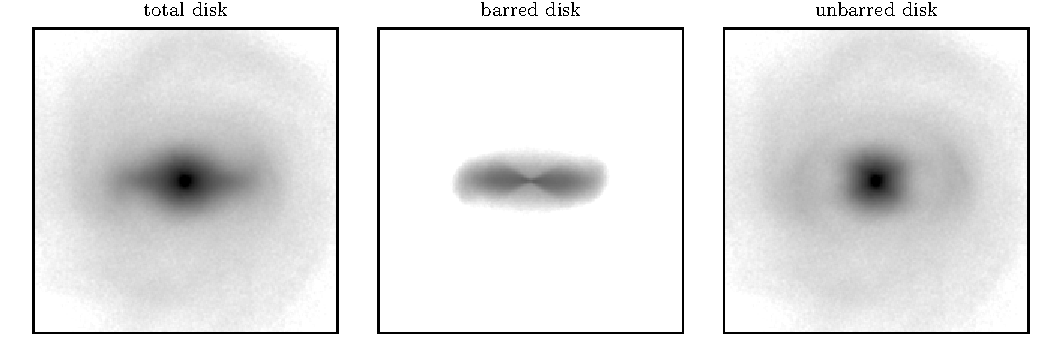
\includegraphics[width=\textwidth]{ch2/fig/bar_decomp.pdf}
    \caption{Disk decomposition into the barred and unbarred disk. This
    procedure is based on \citet{2016MNRAS.463.1952P}. The \textit{left panel}
    shows a face-on surface density projection through the stellar component of
    the \SMUGGLE{} simulation (disk and bulge) at $t=1\,\textrm{Gyr}$. The
    \textit{middle panel} shows the component of the disk identified as being
    trapped in the bar while the \textit{right panel} shows the component of the
    disk identified as not being trapped in the bar. The fact that the untrapped
    stars form a roughly axisymmetric structure indicates our bar decomposition
    is sufficiently accurate. We have computed that $76\%$ of the second Fourier
    component resides in the stars classified as being trapped in the bar.}
    \label{fig:decomp}
\end{figure*}

Computing the length of the bar and the torque on the bar by different
components requires us to decompose the disk into a component which is trapped
by the bar and a component which is untrapped. In order to do this, we follow
closely the technique developed in \citet{2016MNRAS.463.1952P}. We analyzed the
orbit of each star particle (meaning initial disk, bulge, and newly formed
stars) by extracting the $x$-$y$ positions of the apoapse of each in a frame
corotating with the bar, where apoapses are defined as local maxima in $r$. For
each apoapse, we searched for the $19$ closest apoapses in time and applied a
$k$-means clustering algorithm on this set of $20$ points with $k=2$. We then
computed for each of the two clusters the average angle from the bar
$\left<\Delta \phi\right>_{0,1}$, the standard deviation in $R$ of the points
${\sigma_R}_{0,1}$, and the average radius of the cluster
$\left<R\right>_{0,1}$. At each apoapse, a particle was considered to be in the
bar if it met the following criteria:
\begin{equation}
\textrm{max}\left(\left<\Delta \phi\right>_{0,1}\right) < \pi / 8
\end{equation}
\begin{equation}
\frac{{\sigma_R}_0 + {\sigma_R}_1}{\left<R\right>_0 + \left<R\right>_1} < 0.22
\end{equation}
These criterion are slightly different and simplified from the ones used in
\citet{2016MNRAS.463.1952P}, but we found them to empirically work well at
decomposing the disk into a bar and disk component. In Fig.~\ref{fig:decomp}, we
show an example of this decomposition. The \textit{left} panel shows a surface
density projection of the stellar disk and bulge (including newly formed stars)
from the \SMUGGLE{} model after $1\,\text{Gyr}$ of evolution in a frame such that
the bar is aligned with the $x$-axis. The \textit{middle} panel shows a
projection of the subset of stars that are identified as being trapped in the
bar and the \textit{right} panel shows a projection of the stars that are not
identified as being trapped. The fact that the \textit{right} panel is roughly
axisymmetric indicates the bar decomposition is performing adequately.

We computed the second Fourier component $A_2$ for all particles classified as
barred and unbarred. We found that $76\%$ of the total $m=2$ Fourier component
is in the particles classified as barred (i.e.,
$A_{2,\textrm{bar}}/A_{2,\textrm{tot}}\sim0.76$). Some of this is probably
coming from the $m=4$ component (e.g., boxy orbits) being classified as
unbarred, or the presence of weak spiral arms. See also
\citet{2021MNRAS.500..838P} for more details on the orbit family breakdown.

\section{Varying Pattern Speed}
\label{ch2:app:varyps}
When the bar slows down, we argue that this induces a larger positive torque
from the gas phase. Only gas within corotation will flow inwards, while gas
outside corotation will flow outwards \citep{2011MNRAS.415.1027H}. Since the
corotation radius is larger for more slowly rotating bars, it follows that
more slowly rotating bars should be more efficient at driving gas inflows and
thus experience a larger positive torque from the gas phase.

We performed an experiment to test this hypothesis by freezing the stellar
disk in the \SMUGGLE{} run and forcing it to rotate at a constant angular rate.
This has the effect of forcing the bar to rotate as a solid body at a constant
angular rate which we control. The gas is evolved self-consistently with this
rotating disk. We measured the torque on the bar by the gas phase at different
rotation rates. The result of this experiment is illustrated in
Fig.~\ref{fig:equil}, which shows that a more slowly rotating bar experiences a
larger positive torque from the gas.

We also note that since \citet{2011MNRAS.415.1027H} predicts gas outside of
corotation will flow outward, the bar should exert a positive torque on that
gas. Indeed, we measured the average torque on gas outside corotation from
$t=3\,\textrm{Gyr}$ to $5\,\textrm{Gyr}$ to be $0.87$ in code units
($10^{10}\,M_{\odot}\,(\text{km}/\text{s})^2$). For reference, the average
torque inside corotation is $-10.8$ over the same time period and in the same
units. So, while gas outside corotation does experience a positive torque, the
total torque on the gas phase is still negative.

\begin{figure*}
    \centering
    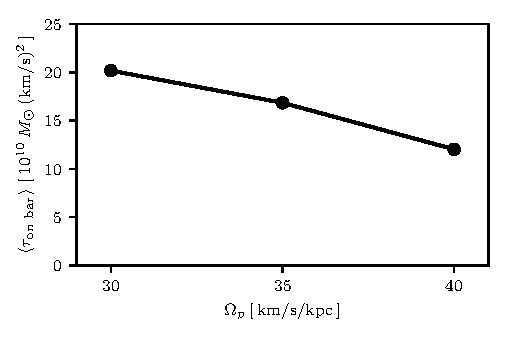
\includegraphics[width=9cm]{ch2/fig/torque_ps.pdf}
    \caption{Average torque exerted by gas on a bar which rotates at a fixed
    pattern speed. Since only gas within the corotation radius is able to infall
    and slower bars have larger corotation radii, slower bars experience a
    larger net torque than faster bars. The setup of the simulations used here
    is identical to the \SMUGGLE{} case discussed earlier, except the \Nbody{} disk
    is rotated as a solid body with a constant angular
    velocity.}
    \label{fig:equil}
\end{figure*}

\begin{figure*}
    \centering
    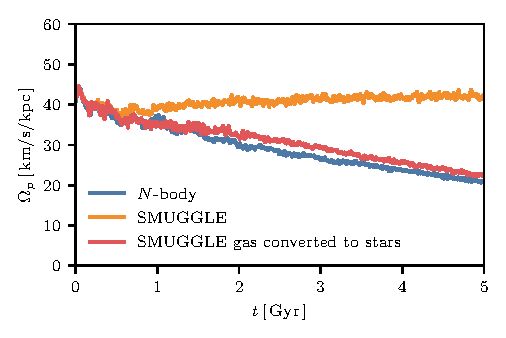
\includegraphics[width=9cm]{ch2/fig/ps_star.pdf}
    \caption{Pattern speed evolution of a model in which we instaneously
    add stars instead of gas to the simulation, with the same density profile as
    the gas phase. The pattern speed evolution in this case is qualitatively
    similar to that of the $N$-body case, with a slight offset in the pattern
    speed. This test demonstrates that the stable pattern speed evolution in the
    SMUGGLE case is not simply a consequence of the change in potential imposed
    in our initial conditions.}
\label{fig:ps-star}
\end{figure*}

\section{Stars Instead of Gas}
In the SMUGGLE model considered in this work, we instantaneously added gas to
the $N$-body system after $1.5\,\textrm{Gyr}$ of evolution. One might wonder if
this sudden change to the potential is responsible for the stable pattern speed
evolution. To test whether this is the case, we added mass to the system in the
same way we did for the SMUGGLE model, but using collisionless particles instead
of gas. The result of this experiment is shown in Fig.~\ref{fig:ps-star}. While
there is an offset compared to the pure $N$-body case, we see that the pattern
speed evolution is broadly consistent with a declining pattern speed. This
indicates that the gas phase is responsible for the stable pattern speed.

\begin{figure}
    \centering
    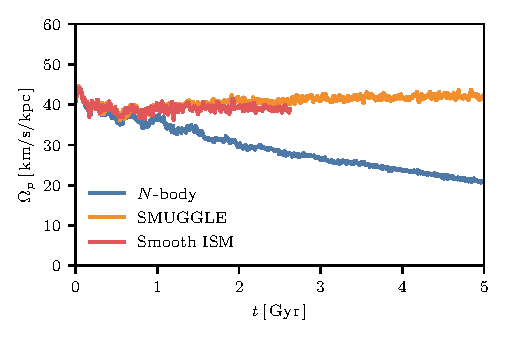
\includegraphics[width=9cm]{ch2/fig/ps_GFM.pdf}
    \caption{Pattern speed evolution of a smooth ISM model. This evolution is
    shown for the fiducial disk in the \Nbody{} (blue), \SMUGGLE{} (orange), and
    smooth ISM (red) cases. The smooth ISM model is an older model for the ISM
    which treats its multiphase nature in a subgrid fashion
    \citep{2003MNRAS.339..289S}. This fundamentally differs from the \SMUGGLE{}
    model, which explicitly resolves the hot and cold phases of the ISM
    \citep{2019MNRAS.489.4233M}. The pattern speed in the smooth ISM case is
    broadly similar to the evolution in the \SMUGGLE{} case. This shows that the
    stability of the pattern speed is not simply a result of our assumed model
    for the ISM.}
\label{fig:GFM}
\end{figure}

\section{Smooth Interstellar Medium}
We performed a simulation of the same disk but with a simpler model of the
interstellar medium \citep{2003MNRAS.339..289S}, closer to standard methods used
in cosmological simulations of galaxy formation and described in more detail in
Section~\ref{ch2:sec:methods}. The result of this test is presented in
Fig.~\ref{fig:GFM}. We find that the pattern speed evolution is nearly the same
in this case, and so conclude that our result is not sensitive to the details of
the model for the interstellar medium.

\section{Semi-Analytic Model Parameters}
\label{ch2:app:sam}
Our semi-analytic model consisted of a three-component bar-disk-halo system. We
describe here the parameters we chose for these components. The parameters of
the disk and halo were chosen to match closely what we used in our fiducial
simulations. The system can thus be understood as being roughly similar to the
Milky Way, though no careful analysis has been performed to ensure the closest
match possible.

For the dark matter halo, we used a Hernquist potential
\citep{1990ApJ...356..359H} with mass $10^{12}\,\Msun$ and a scale length of
$26.2\,\textrm{kpc}$. For the stellar disk, we used a Miyamoto-Nagai disk
\citep{1975PASJ...27..533M} with mass $4.8\times10^{10}\,\Msun$, radial scale
length of $2.67\,\textrm{kpc}$, and vertical scale length of
$0.32\,\textrm{kpc}$. For the bar, we used the quadrupole potential described in
\citet{2022MNRAS.513..768C}. We used their fiducial parameter values --
specifically, we set $A=0.02$, $b=0.28$, and $v_c = 235\,\kms$. Our initial
pattern speed is always set to $40\,\kms/\textrm{kpc}$.

We integrated our model for $5\,\textrm{Gyr}$ with a timestep of
$0.01\,\textrm{Gyr}$.

\section{Comparison to the Milky Way}
\label{ch2:app:milkyway}
For several Gyr, our fiducial disk exhibits several properties in reasonable
agreement to the Milky Way. This is uncommon in models of galaxies that include
the gas phase of the disk but no circumgalactic medium. As mentioned earlier,
the pattern speed seems to match the observed pattern speed of the Milky Way's
bar \citep{2019MNRAS.490.4740B}. We briefly summarize some of the other ways our
disk is comparable to the Milky Way.

We computed the circular velocity curve of our model using the \texttt{AGAMA}
package \citep{2019MNRAS.482.1525V}. We fit the baryonic component (stellar
disk, bulge, gas, and newly formed stars) with an axisymmetric cylindrical
spline with $20$ grid points in both the radial and vertical direction spanning
$0.2$ to $50\,\textrm{kpc}$ in the radial direction and from $0.02$ to
$10\,\textrm{kpc}$ in the vertical direction. We fit the dark matter halo using
an axisymmetric multipole fit with a maximum angular harmonic coefficient
of $l=2$, to account for the compression of the halo by the disk. We plot
the circular velocity curve at $t=1\,\textrm{Gyr}$ in Fig.~\ref{fig:vcirc}
compared to observational estimates \citep{2019ApJ...871..120E}. The \SMUGGLE{}
disk (which includes additional mass in the form of gas) has a slightly higher
circular velocity than the \Nbody{} disk which, itself, is slightly higher than
the observational estimates. Overall, though, the circular velocity curves
between our model and that observed in the Milky Way are broadly consistent.

We also show the evolution of the surface density profile in Fig.~\ref{fig:surf}
We find that in our simulation the atomic and molecular gas surface density and
the SFR surface density is broadly consistent with the expected values for the
Milky Way \citep{2008A&A...487..951K,2022ApJ...929L..18E}. The discrepancy between
$1$ and $4\,\textrm{kpc}$ in the molecular and SFR surface density is probably due
to the fact that the distances to molecular clouds which underlines this work
used a simple kinematic distance based on an axisymmetric model of the Milky
Way \citep{2017ApJ...834...57M}, which is not accurate in the bar region where gas
has large non-circular velocities.

We measured the initial scale height of the atomic gas disk in a bin
extending from $R=7.5\,\textrm{kpc}$ to $R=8.5\,\textrm{kpc}$. The initial
vertical profile is well-fit by a Gaussian with a scale height of
$110\,\textrm{pc}$. At $t=1\,\textrm{Gyr}$, the vertical profile in the same
radial bin is better fit by an exponential profile with scale height of
$74\,\textrm{pc}$. These are somewhat lower than the observed value in the HI
disk of $\sim200\,\textrm{pc}$ \citep{1995ApJ...448..138M, 2017A&A...607A.106M}.
This may be caused by the model in our simulations not driving enough turbulent
pressure, and is an interesting avenue of further investigation.

\begin{figure*}
    \centering
    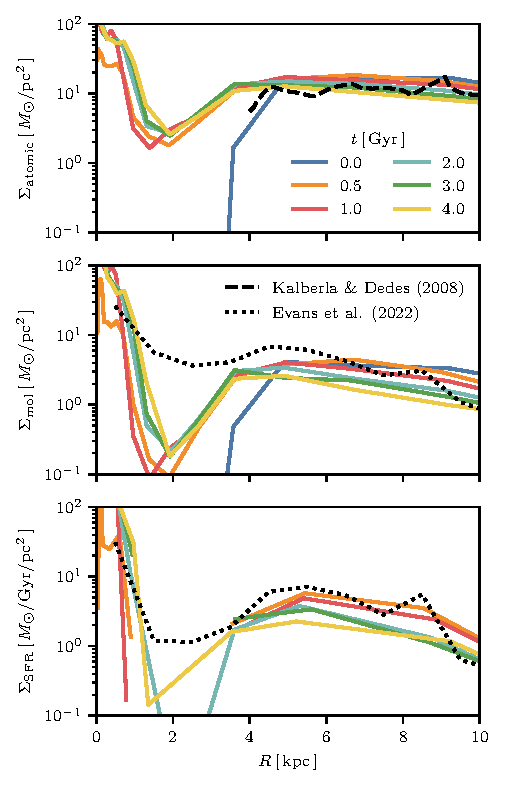
\includegraphics[width=9cm]{ch2/fig/surf_dens.pdf}
    \caption{The time evolution of the atomic gas surface density
    (\textit{upper}), molecular gas surface density (\textit{middle}) and the
    star formation rate (SFR) surface density (\textit{lower}) at various times
    during our fiducial simulation. Colored lines indicate the profiles at
    selected times during the simulation while the black dashed lines indicate
    observations for the atomic gas \citep{2008A&A...487..951K} and black dotted
    lines indicate a model which allows the CO-to-H$_2$ conversion factor
    $X_{\textrm{CO}}$ to vary with metallicity \citep{2022ApJ...929L..18E}.
    Molecular gas surface densities were provided separately (N. Evans, private
    communication). We see that the molecular gas and SFR surface densities are
    within an order of magnitude of the Milky Way's typical values at all times.
    We see a sharp decrease in the gas and SFR surface densities along the
    extent of the bar from $\sim1$ to $\sim4\,\textrm{kpc}$, related to the gas
    inflow in this region.}
    \label{fig:surf}
\end{figure*}

\begin{figure}
    \centering
    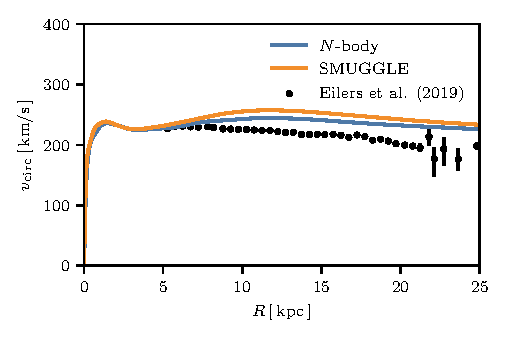
\includegraphics[width=9cm]{ch2/fig/vcirc.pdf}
    \caption{The circular velocity curve of our setups at $t=1\,\textrm{Gyr}$.
    This curve is shown for the \Nbody{} run (blue) and the \SMUGGLE{} run
    (orange) compared to observational estimates for the Milky Way
    \citep{2019ApJ...871..120E}. We see that the circular velocity curve for
    both runs is marginally larger than the Milky Way's, but still comparable.
    The \SMUGGLE{} circular velocity curve is larger than the \Nbody{} curve due
    to the additional mass in the gas phase.}
    \label{fig:vcirc}
\end{figure}

\chapter{Appendix to Chapter~\ref{ch:GSEgas}}\label{ch:app_GSEgas}

\section{Star Formation Histories}\label{ch3:app:all_sfh}
One potential avenue for creating an \FeH{}-dependent star formation gap is through quiescence. This is demonstrated by examining the global SFH in Figure~\ref{fig:all_sfh}, with the panels and colors showing each simulation in the grid ordered by their bimodality score $\mathcal{B}$ in the same way as Figures~\ref{ch3:fig:all_hist} and \ref{ch3:fig:all_scatter}. One can see that there is a global quiescent period in simulations~g, s, and x. Simulations~s and x have a bimodal pattern, while simulation~g has a unimodal pattern. As mentioned in Figure~\ref{ch3:fig:all_scatter}, simulation~g has an age gap but there is not enough star formation at $\FeH\sim0$ before the gap to result in a strong bimodality. Otherwise, while a global quiescent period is sufficient for generating an age gap, most simulations do not have a global quiescent period.

\begin{figure*}
  \centering
  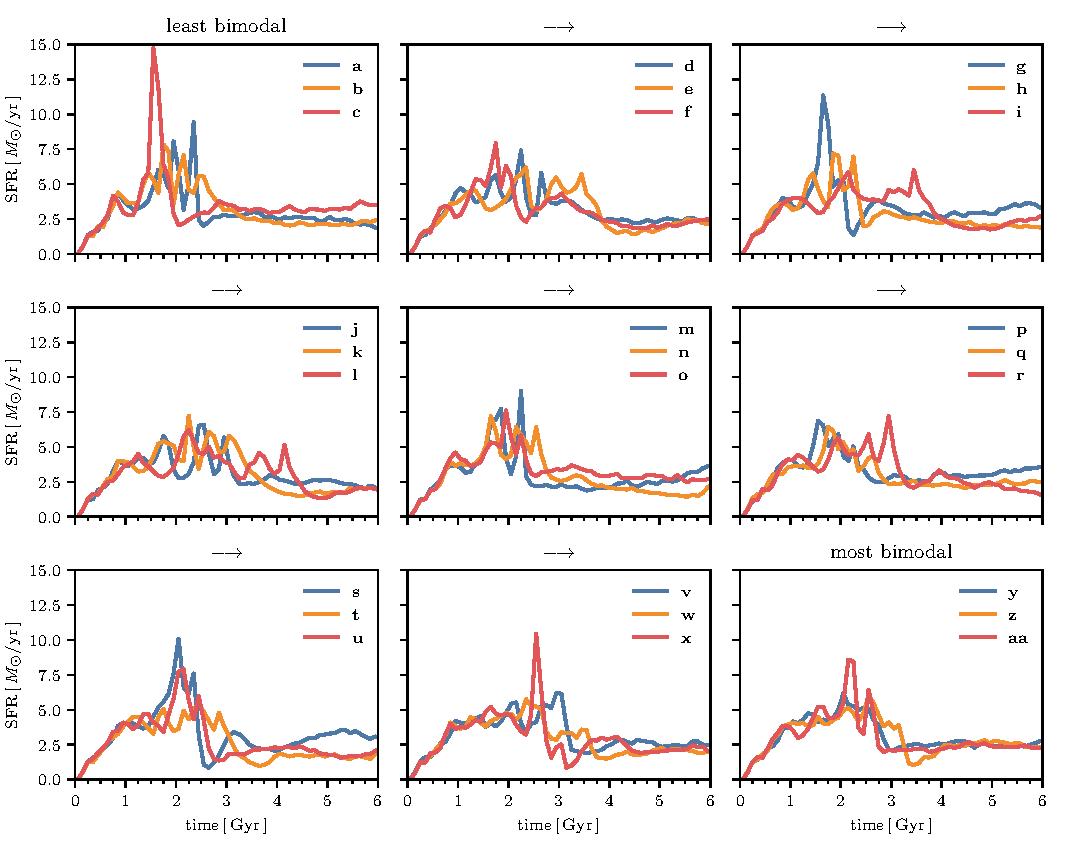
\includegraphics[width=\textwidth]{ch3/sfh.pdf}
  \caption{Global star formation history (SFH) for each simulation, plotted in the same order as Figures~\ref{ch3:fig:all_hist} and \ref{ch3:fig:all_scatter}, with increasing bimodality score $\mathcal{B}$ from left to right. The colors correspond to the same simulations as in previous figures. A global quiescent period, characterized by a significant dip in the SFR, is observed in simulations~g, s, and x. Among these, simulations~s and x exhibit strong bimodal \MgFe{} distributions, while simulation~g remains unimodal due to insufficient early star formation at $\FeH\sim0$ before the quiescent phase. Most other simulations do not display a clear global quiescent period, indicating that such a phase is not strictly necessary for bimodality to emerge.}
  \label{fig:all_sfh}
\end{figure*}

\section{Cause of Suppressed Star Formation}\label{ch3:app:cause_qui}
In Figure~\ref{fig:MdotBH_rsep}, we demonstrate how the orbit of the bimodal simulation is closely related to the strength of BH feedback. On the $y$-axis, we show in blue the black hole accretion rate as a ratio of the maximum (Eddington) accretion rate at that time. In orange we show the orbital separation between the satellite and central galaxies. We see that the accretion rate is high early on at $\sim10\%$. At the time around coalescence at $\sim2\,\Gyr$, the accretion rate rises up to Eddington, before dropping to a much lower value $<10\%$ later on.

In the TNG model, the strength of AGN feedback is directly tied to the BH's accretion rate \citep{2017MNRAS.465.3291W}. Therefore, it is reasonable to suspect that the feedback from the AGN is responsible for removing gas from the galaxy or keeping it above the star forming density threshold.

\begin{figure}
  \centering
  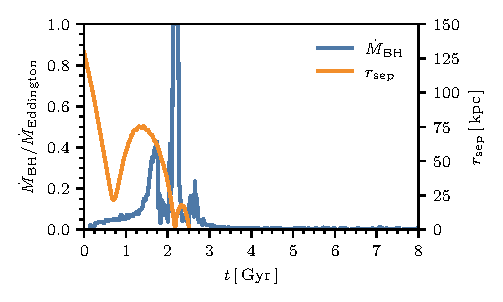
\includegraphics[width=242.26653pt]{ch3/MdotBH_rsep.pdf}
  \caption{Evolution of black hole accretion rate and orbital separation over time in the bimodal simulation. The blue line shows the black hole accretion rate as a fraction of the Eddington rate, while the orange line shows the orbital separation between the satellite and central galaxies. The accretion rate peaks during coalescence at $\sim2\,\Gyr$, suggesting a strong connection between the merger and AGN activity.}
  \label{fig:MdotBH_rsep}
\end{figure}

\section{Abundance Plane of All Simulations}\label{ch3:app:allmerge}
We show summary plots of the abundance planes of all simulations in our orbital grid in Figures~\ref{fig:allmerge0} to \ref{fig:allmerge8}.

\begin{figure*}
  \centering
  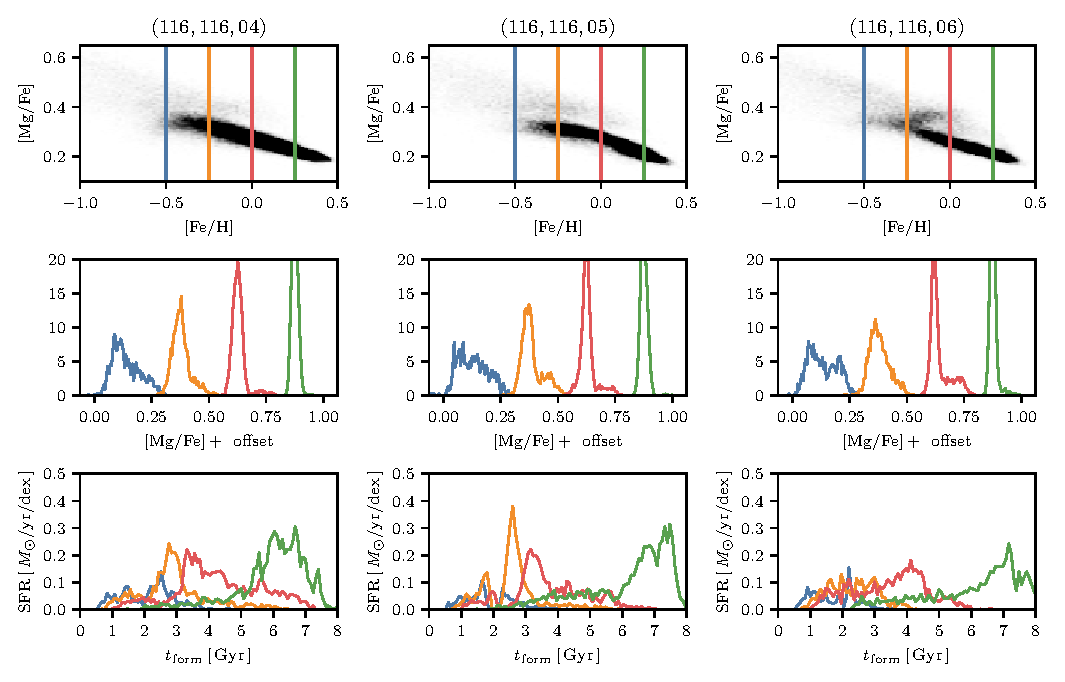
\includegraphics[width=\textwidth]{ch3/allmerge0.pdf}
  \caption{A summary of the abundance plane and star formation history of all simulations within the orbital grid. Each figure shows the outcome of a simulation at a fixed $R_0$ and $V_0$, varying $\eta$. The title of each column shows the $R_0$, $V_0$, and $\eta$ of that simulation, in order. The upper and middle rows replicate Figure~\ref{ch3:fig:fig1}, which show the distribution of stars in the abundance plane of \MgFe{}-\FeH{} as well as 1D histograms at a fixed \FeH{} of $-0.5$, $-0.25$, $0$, and $0.25$. The lower rows replicate Figure~\ref{ch3:fig:before_after_sfh_by_iron}, showing the star formation history at each \FeH{}.}
  \label{fig:allmerge0}
\end{figure*}

\begin{figure*}
  \centering
  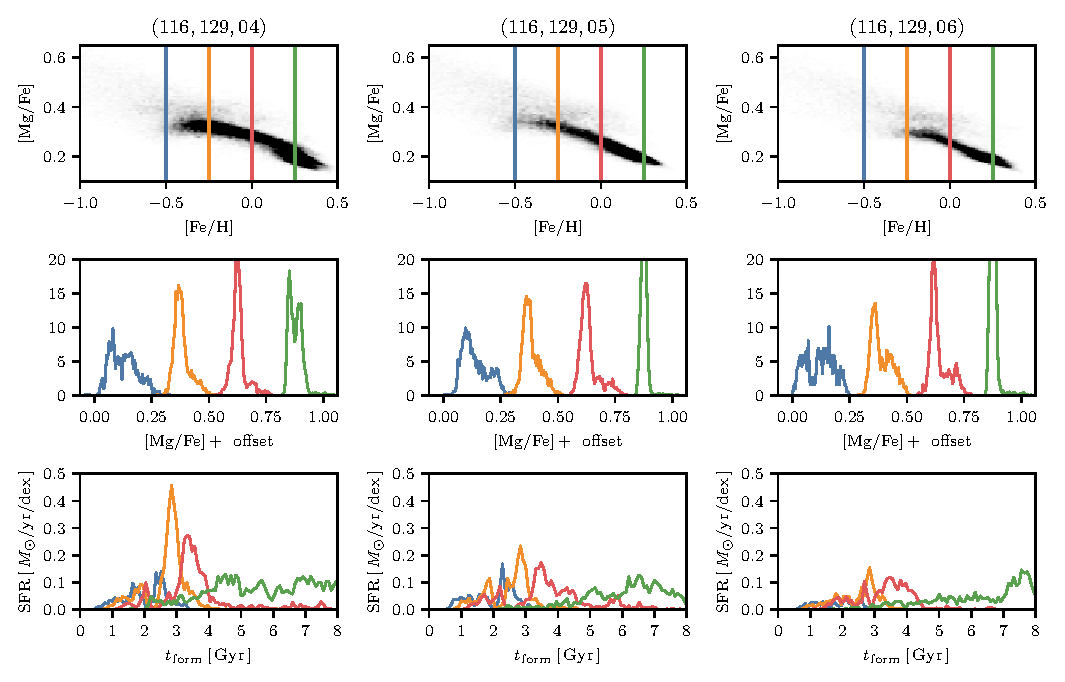
\includegraphics[width=\textwidth]{ch3/allmerge1.pdf}
  \caption{A continuation of Figure~\ref{fig:allmerge0}.}
  \label{fig:allmerge1}
\end{figure*}

\begin{figure*}
  \centering
  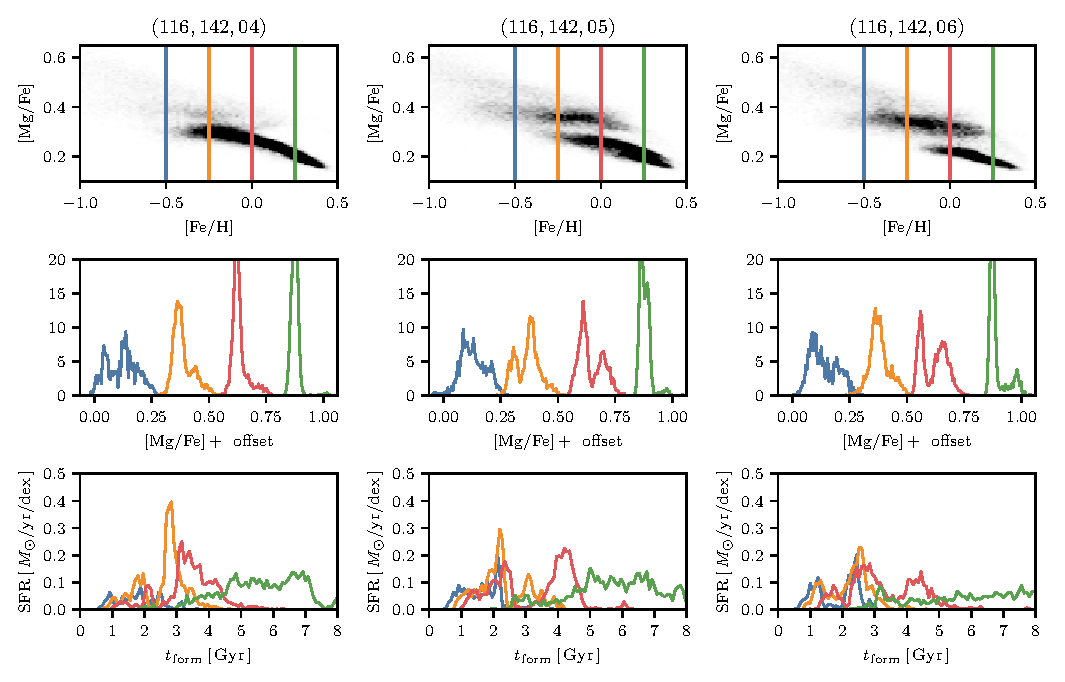
\includegraphics[width=\textwidth]{ch3/allmerge2.pdf}
  \caption{A continuation of Figure~\ref{fig:allmerge0}.}
  \label{fig:allmerge2}
\end{figure*}

\begin{figure*}
  \centering
  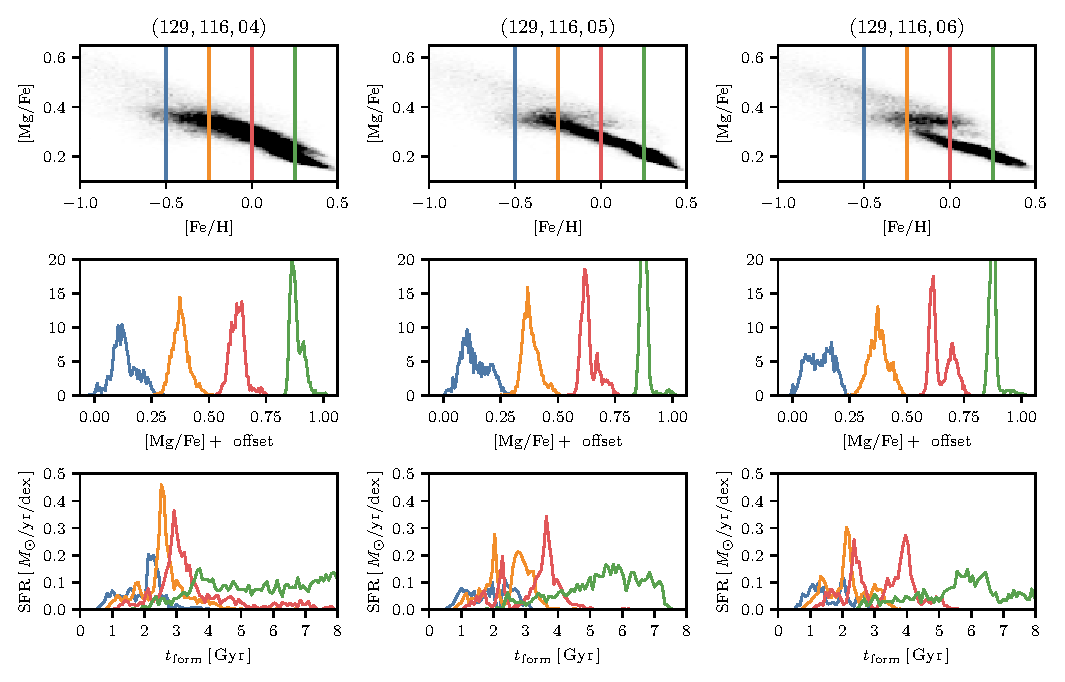
\includegraphics[width=\textwidth]{ch3/allmerge3.pdf}
  \caption{A continuation of Figure~\ref{fig:allmerge0}.}
  \label{fig:allmerge3}
\end{figure*}

\begin{figure*}
  \centering
  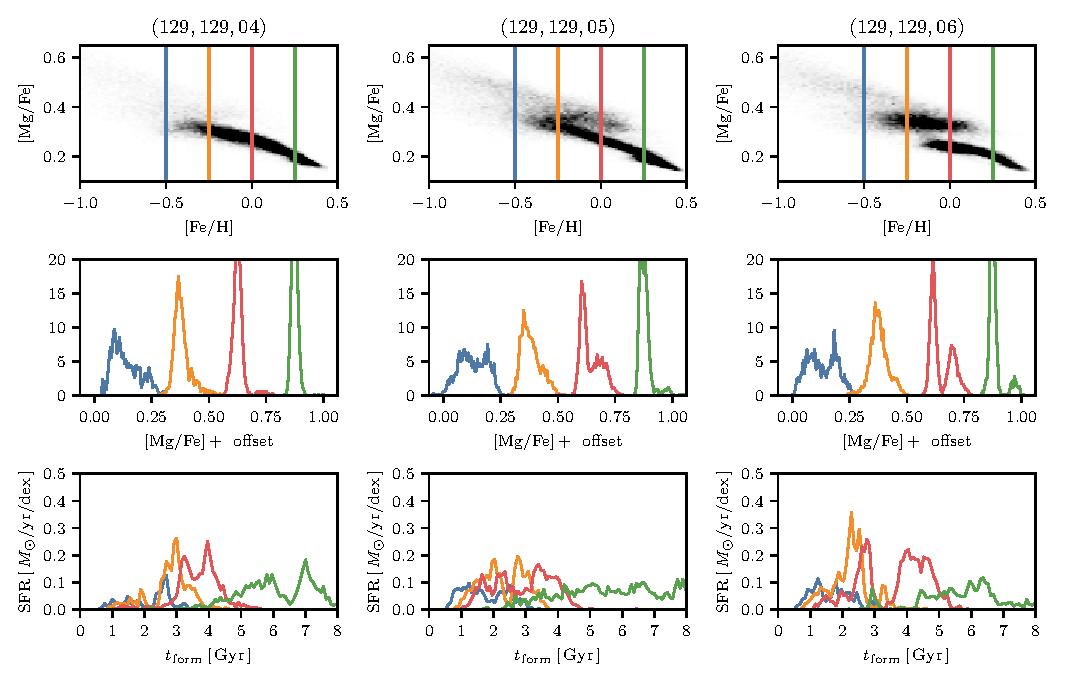
\includegraphics[width=\textwidth]{ch3/allmerge4.pdf}
  \caption{A continuation of Figure~\ref{fig:allmerge0}.}
  \label{fig:allmerge4}
\end{figure*}

\begin{figure*}
  \centering
  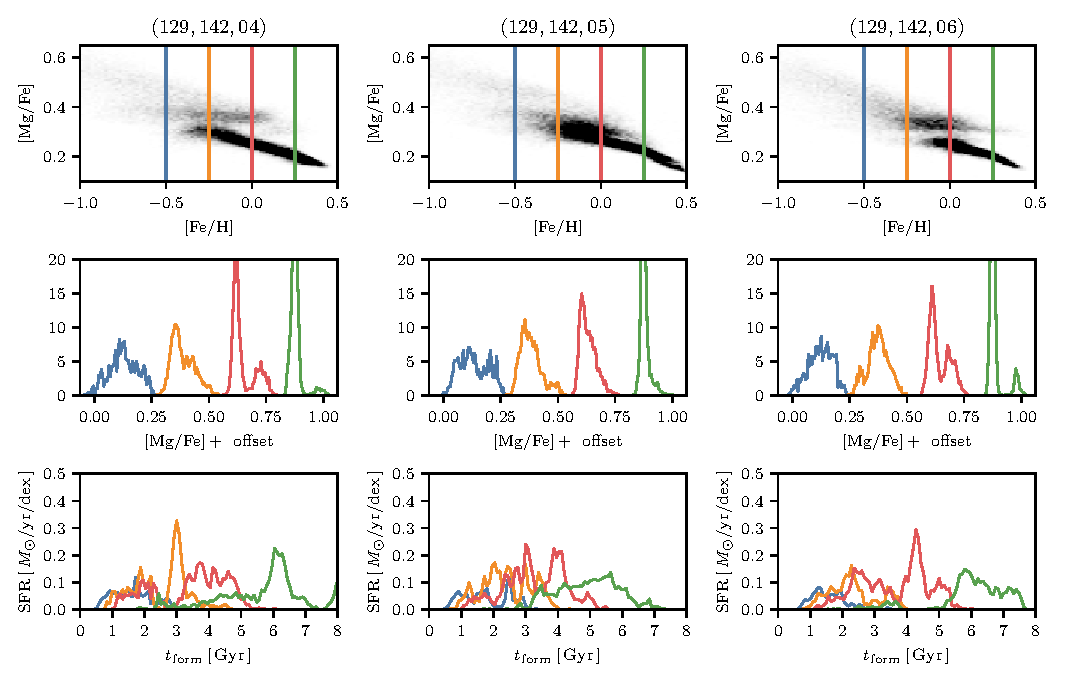
\includegraphics[width=\textwidth]{ch3/allmerge5.pdf}
  \caption{A continuation of Figure~\ref{fig:allmerge0}.}
  \label{fig:allmerge5}
\end{figure*}

\begin{figure*}
  \centering
  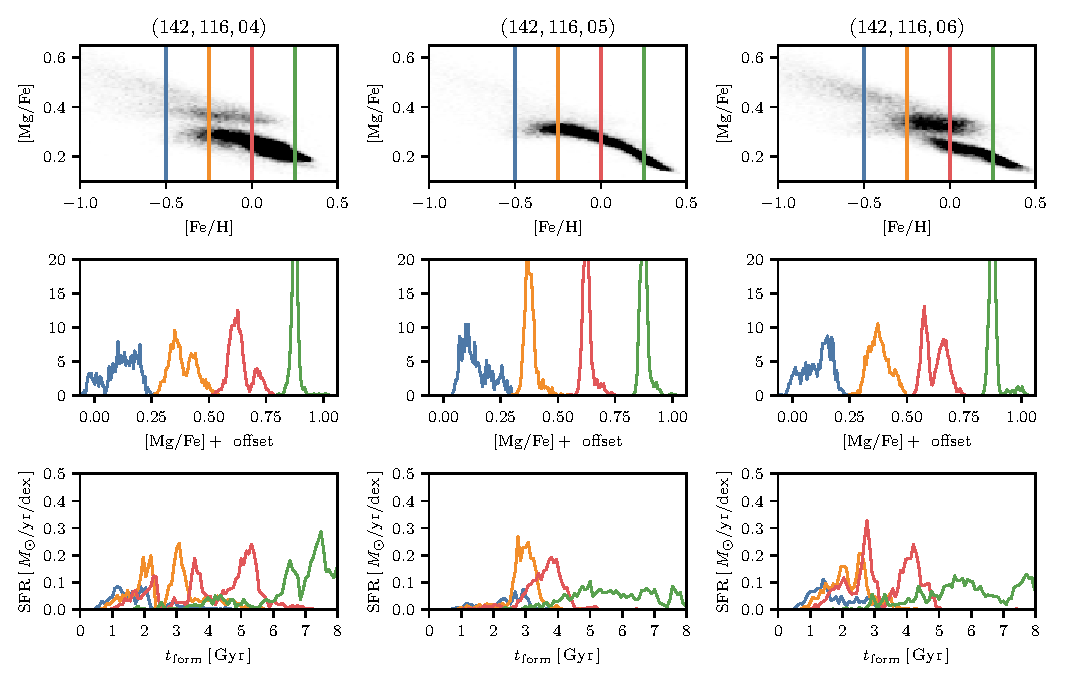
\includegraphics[width=\textwidth]{ch3/allmerge6.pdf}
  \caption{A continuation of Figure~\ref{fig:allmerge0}.}
  \label{fig:allmerge6}
\end{figure*}

\begin{figure*}
  \centering
  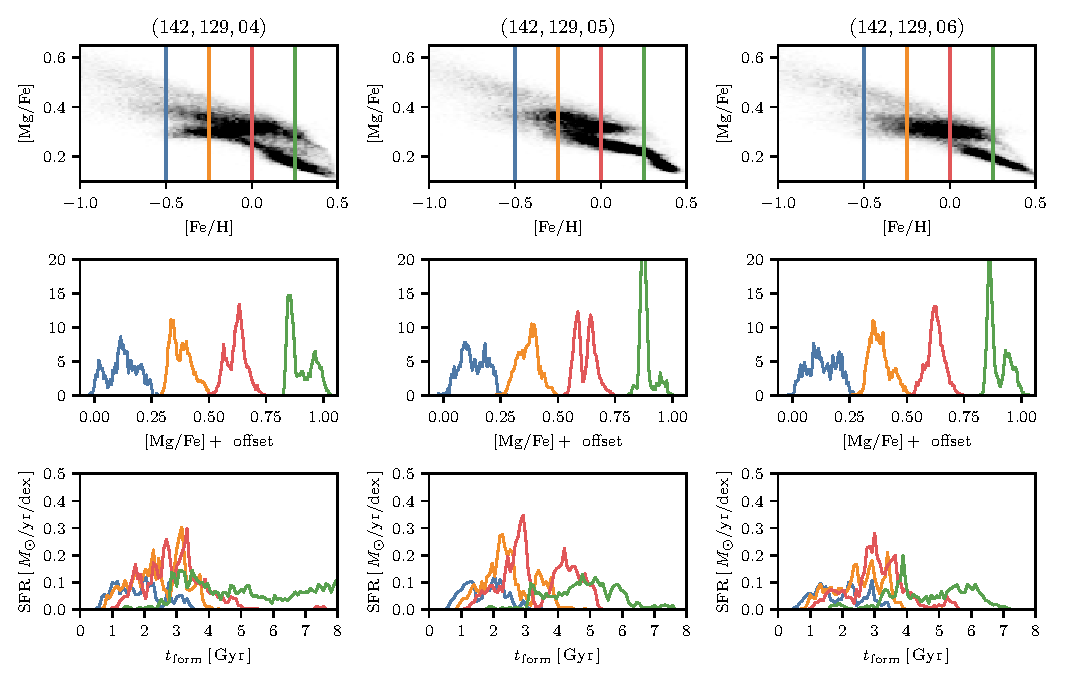
\includegraphics[width=\textwidth]{ch3/allmerge7.pdf}
  \caption{A continuation of Figure~\ref{fig:allmerge0}.}
  \label{fig:allmerge7}
\end{figure*}

\begin{figure*}
  \centering
  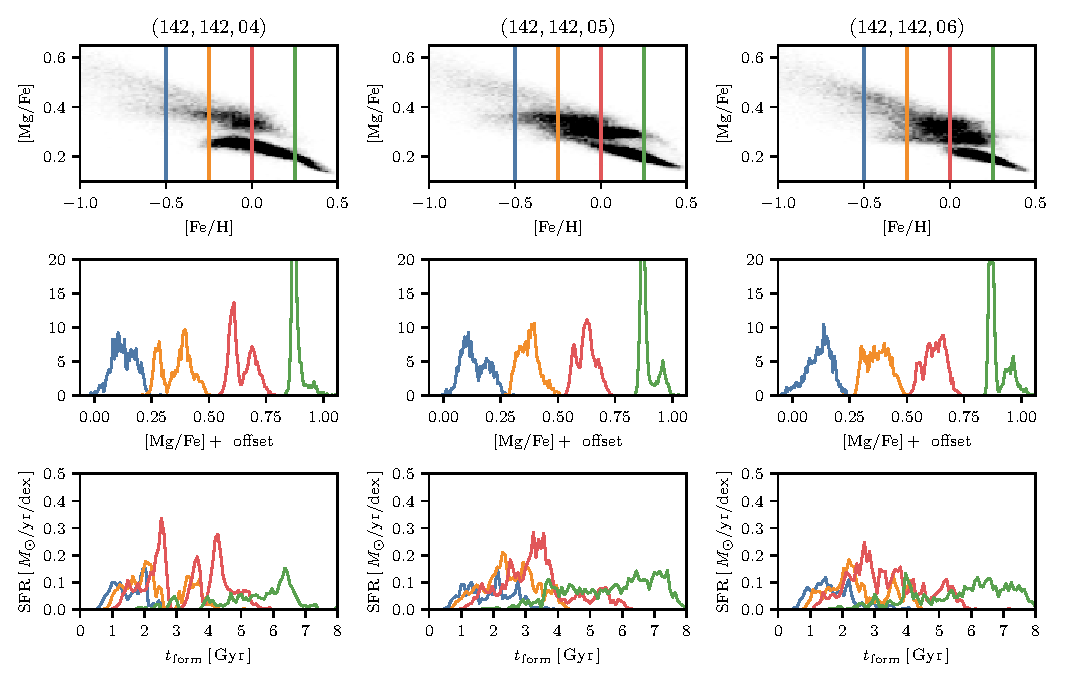
\includegraphics[width=\textwidth]{ch3/allmerge8.pdf}
  \caption{A continuation of Figure~\ref{fig:allmerge0}.}
  \label{fig:allmerge8}
\end{figure*}

\chapter{Appendix to Chapter~\ref{ch:Mgdec}}\label{ch:app_Mgdec}
\section{Observational Errors}\label{ch4:app:obs_err}
In Figure~\ref{fig:alpha}, we assumed observational errors of $12.5\%$ in age and $0.015\,\dex$ in \MgFe{}. In Figure~\ref{fig:obs_err}, we plot the quoted observational errors of the APOKASC-3 (left) and ASPCAP (right) datasets, showing both \FeH{} and \MgFe{} (blue and orange, respectively). We show our $12.5\%$ age error as a black line in the left panel. We take the age error to be the maximum of the upper and lower errors from \citet{2018ApJS..239...32P}. In the right panel, we show blue and orange vertical lines at $0.01$ and $0.015\,\dex$ for \FeH{} and \MgFe{}, respectively. These are approximately the 99th percentiles of each error distribution. As a dashed line we show our $25\%$ age error cut for stars plotted in Figure~\ref{fig:obs_err}. Our assumed errors are generally consistent with the errors quoted in the dataset, with a conservative estimate for the abundance errors.

\begin{figure*}
  \centering
  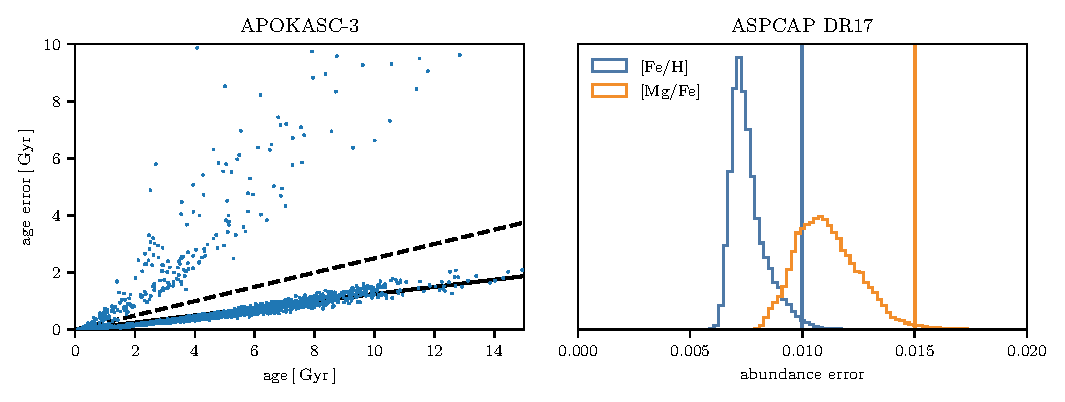
\includegraphics[width=\columnwidth]{ch4/obs_error.pdf}
  \caption{The observational errors of astroseismic ages from APOKASC-3 (left) and abundances from ASPCAP DR17 (right). We show, on the left, a line indicating a $12.5\%$ error in observed age and on the right a vertical line indicating a $0.01$ and $0.015\,\dex$ error in \FeH{} and \MgFe{}, respectively. On the left, a dashed line indicates the $25\%$ error cut used for inclusion in Figure~\ref{fig:alpha}.}
  \label{fig:obs_err}
\end{figure*}

\section{Random Selection of Subhalos}\label{ch4:app:rand_fig1}
In Figure~\ref{fig:app0}, we show the abundance plane of our fiducial galaxy at $z=0$. This reproduces the middle column of Figure~\ref{fig:fig1}. We also show the effect of our $\alpha$-enhancement procedure on this distribution when applied, from left to right, at redshifts of $1$, $1.5$, and $2$. (The $z=1.5$ column reproduces the right column of Figure~\ref{fig:fig1}). Qualitatively, the time at which the $\alpha$-enhancement is applied does not alter whether substructure arises in this plane. However, when it is applied at lower $z$, the peaks between modes do appear to be slightly further apart.

We show the same figure but with an additional random selection of 16 galaxies in the Milky Way-progenitor mass sample as a figure set (17 images), which is available in the online journal. Six additional galaxies (143882, 167392, 348901, 425719, 439099, and 465255) display bimodalities, though none as prominent as the main galaxy studied in this work. Some substructure is present in many galaxies. In general, the $\alpha$-enhancement increases the strength of substructure in the abundance planes. The fact that bimodalities like in the main galaxy studied in this work do not universally appear in $\alpha$-enhanced galaxies indicates that the $\alpha$-enhancement is not solely responsible for the bimodality.

The timing of the $\alpha$-enhancement does not have a major effect on our fiducial galaxy (Figure~\ref{fig:app0}). However, for some (e.g., the green $\FeH=-0.25$ bin in 439099), structure arises only when the $\alpha$-enhancement is applied at sufficiently low redshift. We interpret this as the presence of some substructure inducing activity between $z=1$ and 2.

\begin{figure*}
  \centering
  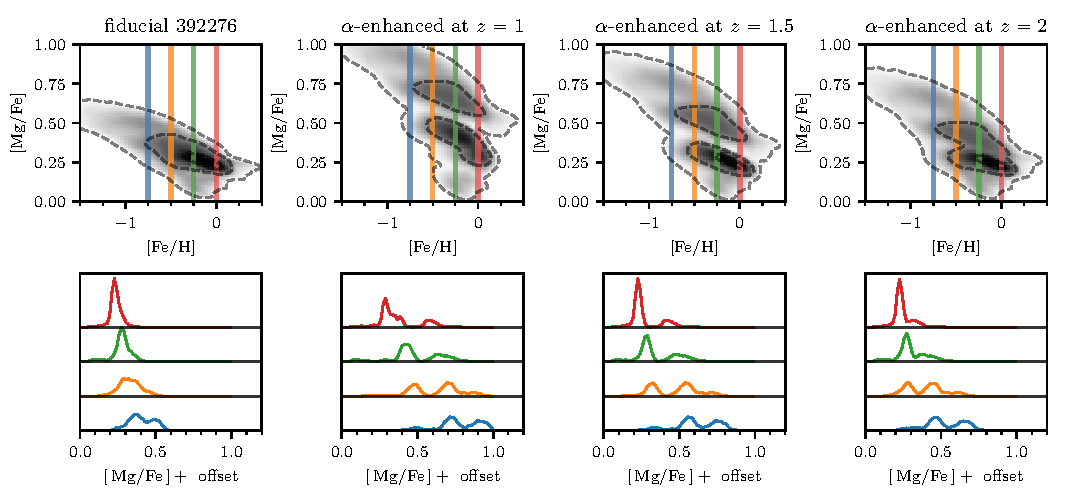
\includegraphics[width=\textwidth]{ch4/app_392276.pdf}
  \caption{Abundance plane of the fiducial galaxy at $z=0$ and the effects of $\alpha$-enhancement applied at different redshifts. The leftmost panel shows the fiducial galaxy without enhancement, reproducing the middle column of Figure~\ref{fig:fig1}. The subsequent panels from left to right show the results of applying $\alpha$-enhancement at redshifts of 1, 1.5, and 2, respectively. The $z=1.5$ column reproduces the right column of Figure~\ref{fig:fig1}. The presence of substructure in the abundance plane is consistent across different application times of $\alpha$-enhancement, though applying it at lower redshifts appears to slightly increase the separation between modal peaks. This figure is part of a set of 17 images available in the online journal, showing similar plots for 16 additional galaxies from our Milky Way-progenitor mass sample. The varied responses to $\alpha$-enhancement across the sample, with only six additional galaxies (143882, 167392, 348901, 425719, 439099, and 465255) displaying bimodalities, suggest that while $\alpha$-enhancement generally increases substructure, it is not solely responsible for creating bimodalities in abundance planes.}
  \label{fig:app0}
\end{figure*}

\begin{figure*}
  \centering
  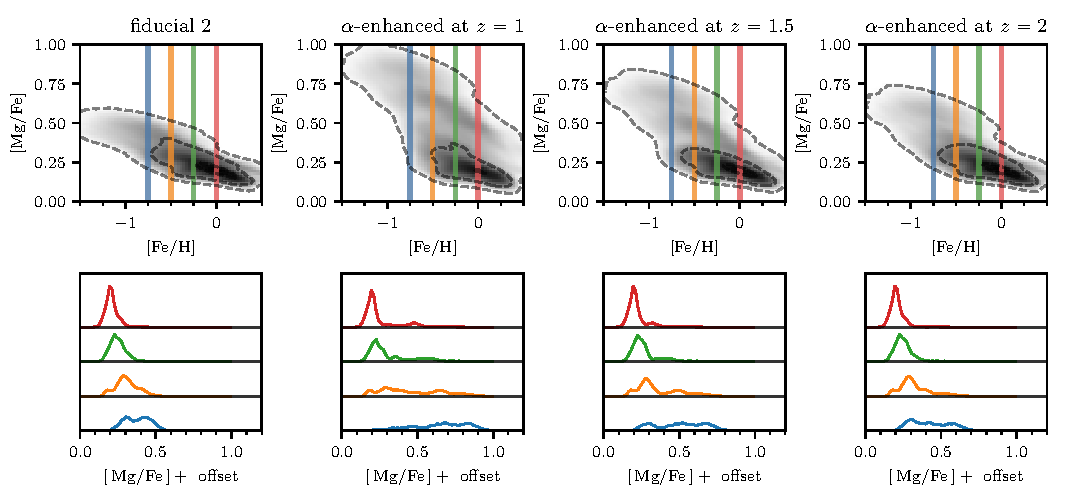
\includegraphics[width=\textwidth]{ch4/app_2.pdf}
  \caption{The same as Figure~\ref{fig:app0}, but for a random galaxy from our initial catalog.}
  \label{fig:app1}
\end{figure*}

\begin{figure*}
  \centering
  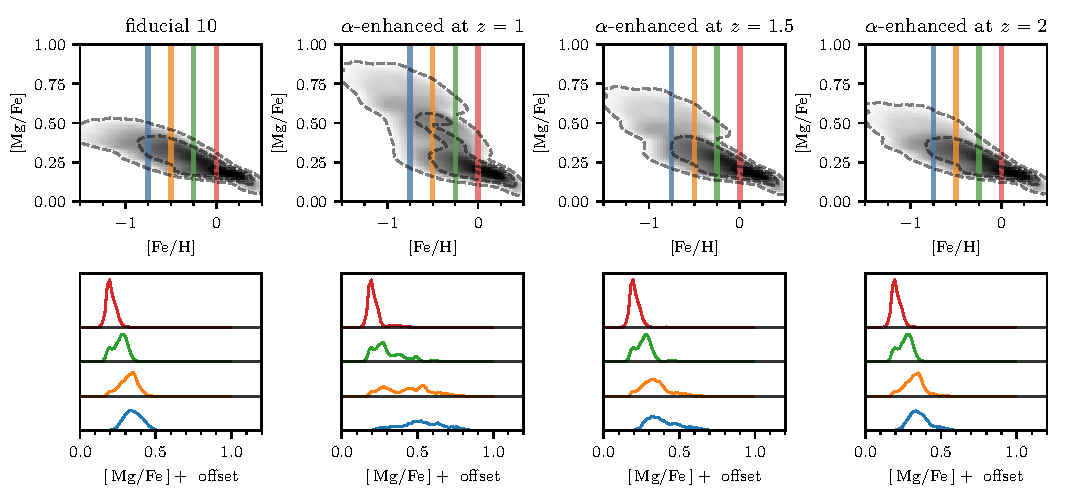
\includegraphics[width=\textwidth]{ch4/app_10.pdf}
  \caption{The same as Figure~\ref{fig:app0}, but for a random galaxy from our initial catalog.}
  \label{fig:app2}
\end{figure*}

\begin{figure*}
  \centering
  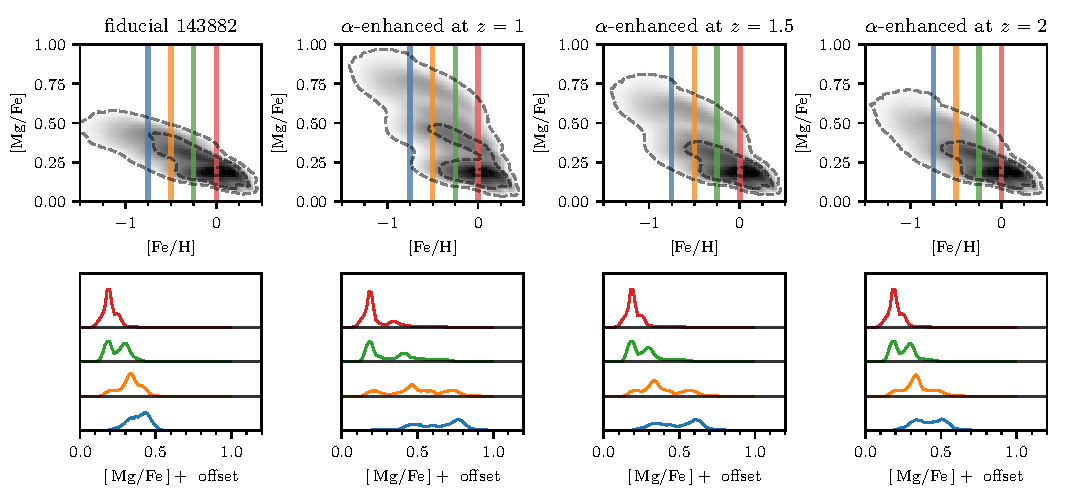
\includegraphics[width=\textwidth]{ch4/app_143882.pdf}
  \caption{The same as Figure~\ref{fig:app0}, but for a random galaxy from our initial catalog.}
  \label{fig:app3}
\end{figure*}

\begin{figure*}
  \centering
  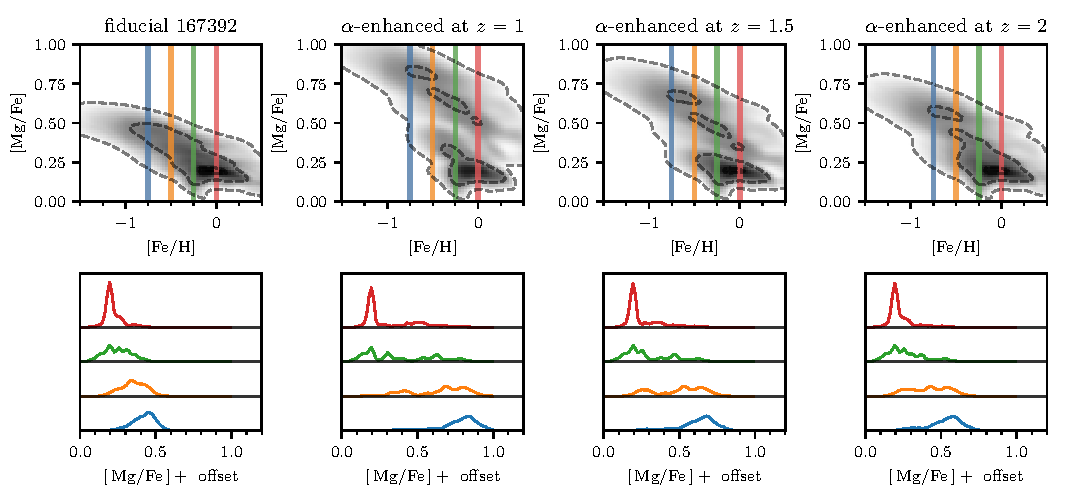
\includegraphics[width=\textwidth]{ch4/app_167392.pdf}
  \caption{The same as Figure~\ref{fig:app0}, but for a random galaxy from our initial catalog.}
  \label{fig:app4}
\end{figure*}

\begin{figure*}
  \centering
  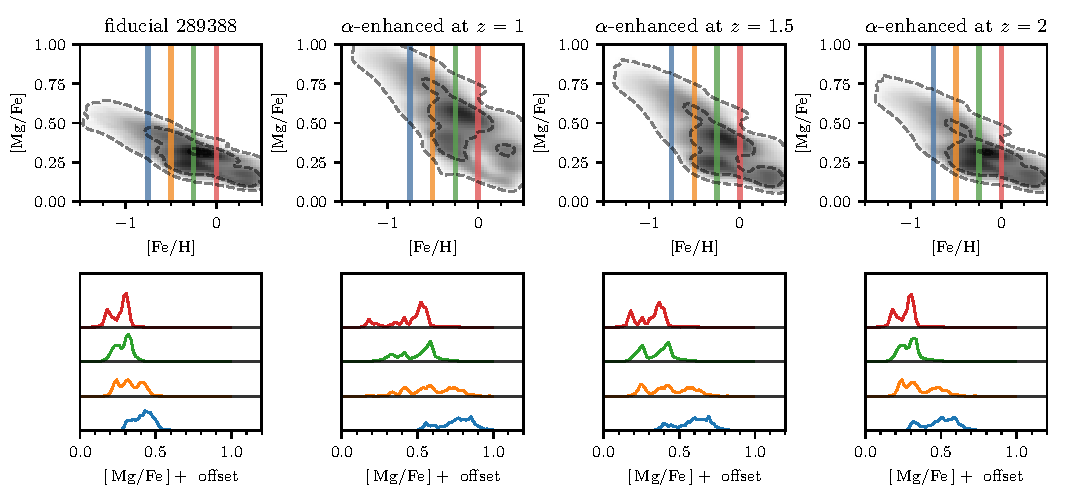
\includegraphics[width=\textwidth]{ch4/app_289388.pdf}
  \caption{The same as Figure~\ref{fig:app0}, but for a random galaxy from our initial catalog.}
  \label{fig:app5}
\end{figure*}

\begin{figure*}
  \centering
  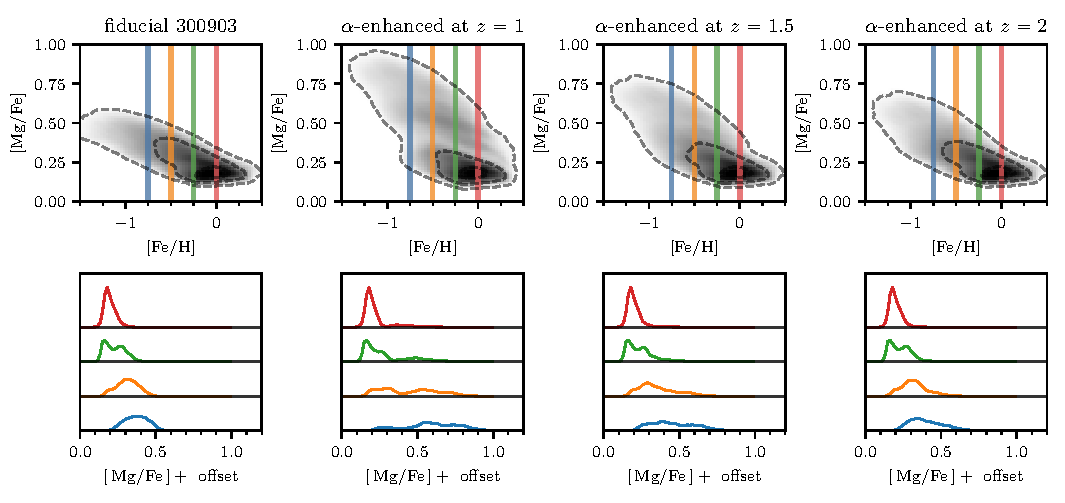
\includegraphics[width=\textwidth]{ch4/app_300903.pdf}
  \caption{The same as Figure~\ref{fig:app0}, but for a random galaxy from our initial catalog.}
  \label{fig:app6}
\end{figure*}

\begin{figure*}
  \centering
  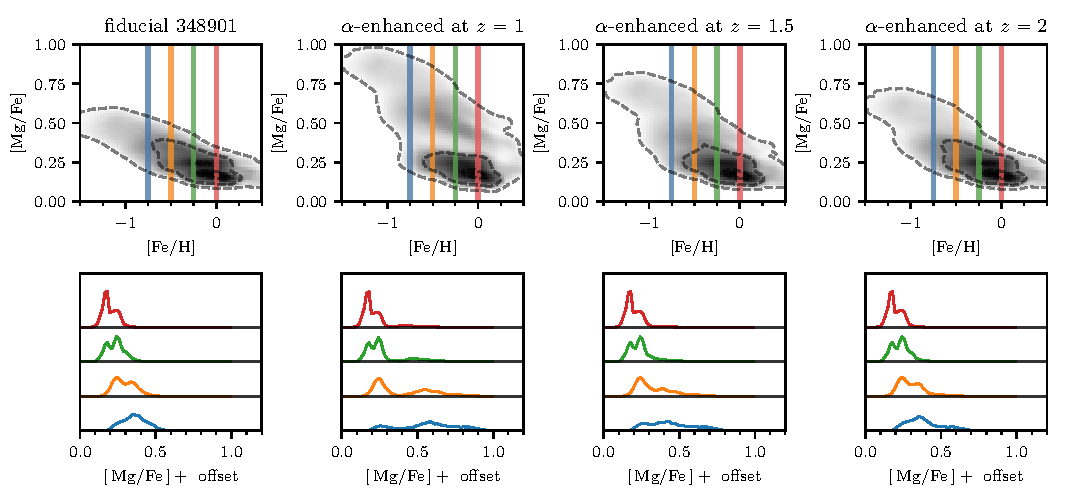
\includegraphics[width=\textwidth]{ch4/app_348901.pdf}
  \caption{The same as Figure~\ref{fig:app0}, but for a random galaxy from our initial catalog.}
  \label{fig:app7}
\end{figure*}

\begin{figure*}
  \centering
  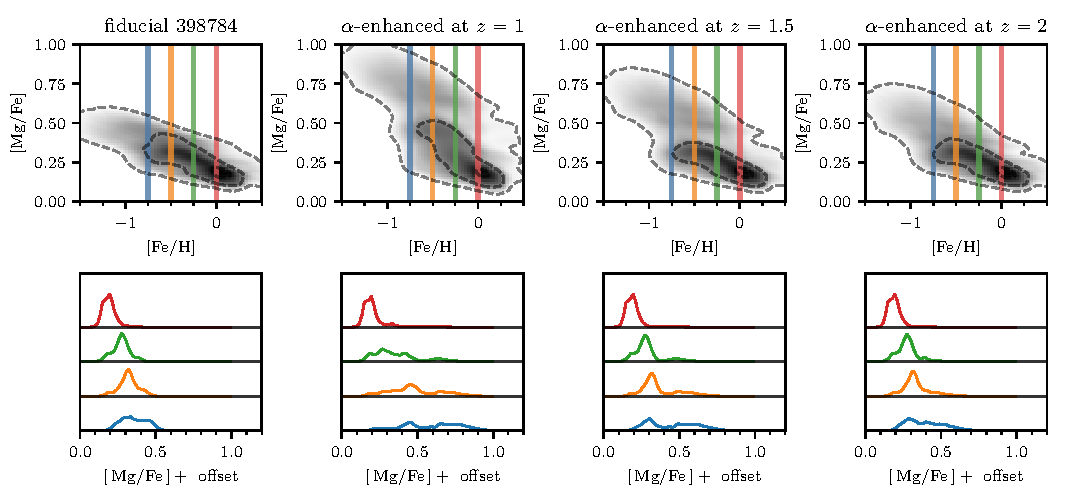
\includegraphics[width=\textwidth]{ch4/app_398784.pdf}
  \caption{The same as Figure~\ref{fig:app0}, but for a random galaxy from our initial catalog.}
  \label{fig:app8}
\end{figure*}

\begin{figure*}
  \centering
  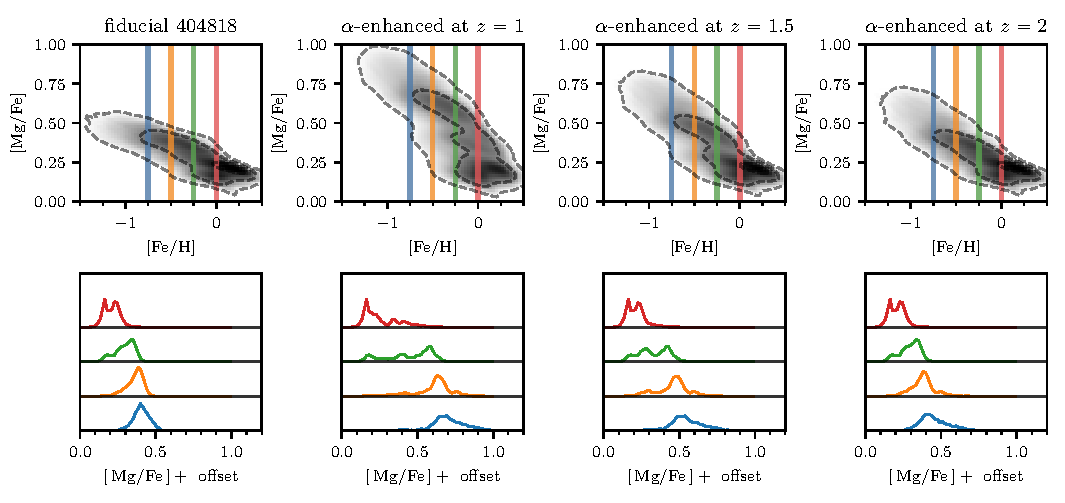
\includegraphics[width=\textwidth]{ch4/app_404818.pdf}
  \caption{The same as Figure~\ref{fig:app0}, but for a random galaxy from our initial catalog.}
  \label{fig:app9}
\end{figure*}

\begin{figure*}
  \centering
  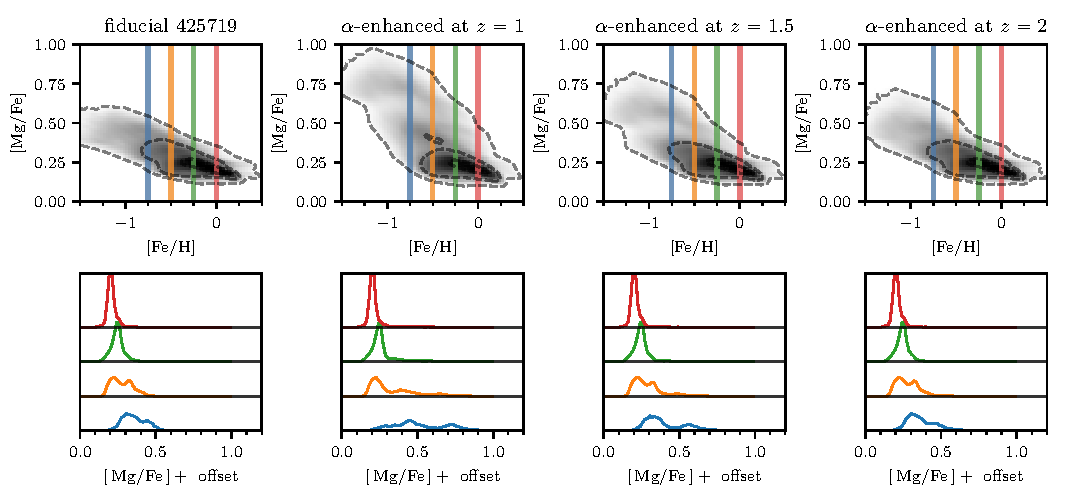
\includegraphics[width=\textwidth]{ch4/app_425719.pdf}
  \caption{The same as Figure~\ref{fig:app0}, but for a random galaxy from our initial catalog.}
  \label{fig:app10}
\end{figure*}

\begin{figure*}
  \centering
  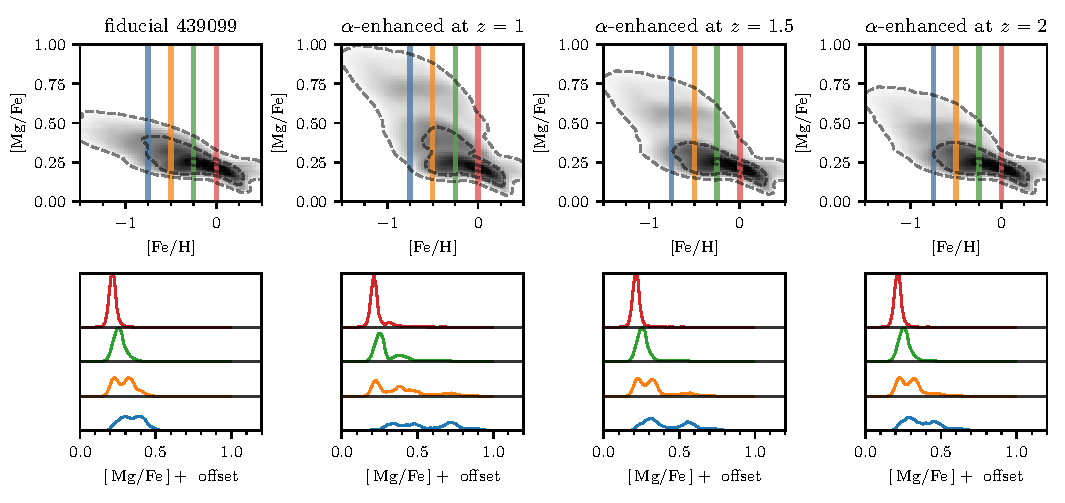
\includegraphics[width=\textwidth]{ch4/app_439099.pdf}
  \caption{The same as Figure~\ref{fig:app0}, but for a random galaxy from our initial catalog.}
  \label{fig:app11}
\end{figure*}

\begin{figure*}
  \centering
  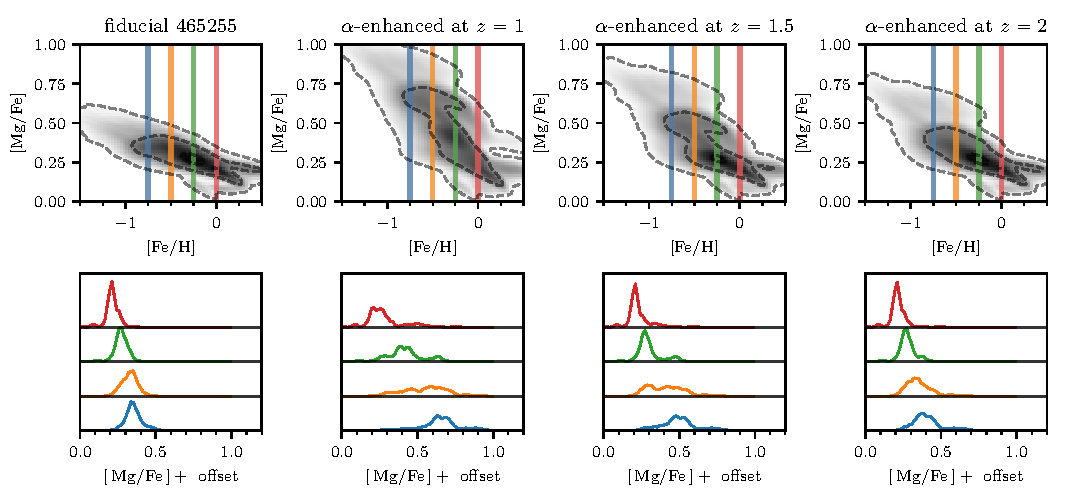
\includegraphics[width=\textwidth]{ch4/app_465255.pdf}
  \caption{The same as Figure~\ref{fig:app0}, but for a random galaxy from our initial catalog.}
  \label{fig:app12}
\end{figure*}

\begin{figure*}
  \centering
  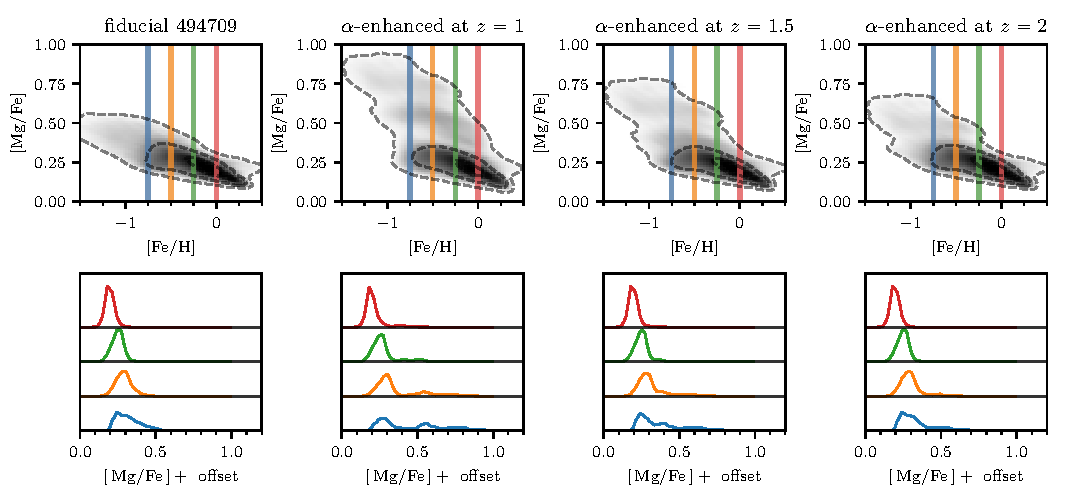
\includegraphics[width=\textwidth]{ch4/app_494709.pdf}
  \caption{The same as Figure~\ref{fig:app0}, but for a random galaxy from our initial catalog.}
  \label{fig:app13}
\end{figure*}

\begin{figure*}
  \centering
  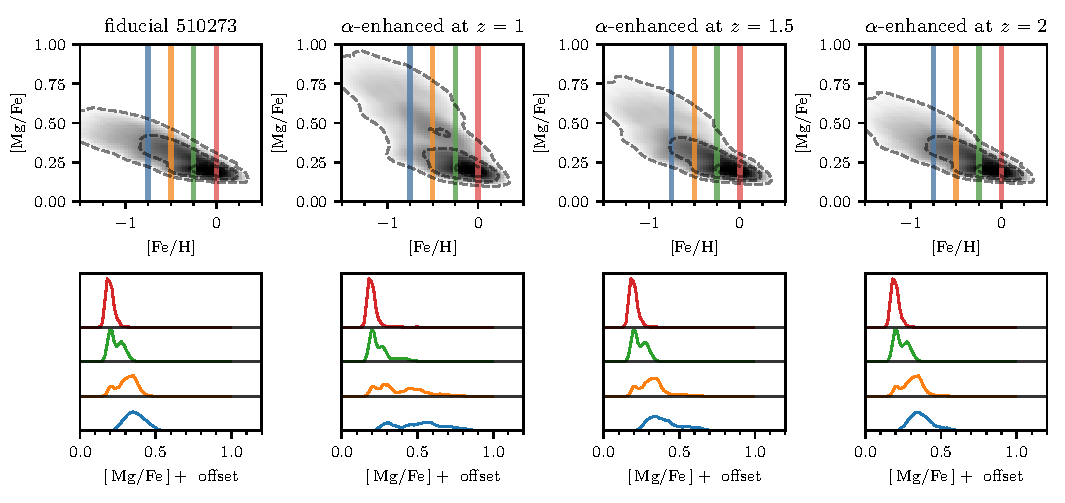
\includegraphics[width=\textwidth]{ch4/app_510273.pdf}
  \caption{The same as Figure~\ref{fig:app0}, but for a random galaxy from our initial catalog.}
  \label{fig:app14}
\end{figure*}

\begin{figure*}
  \centering
  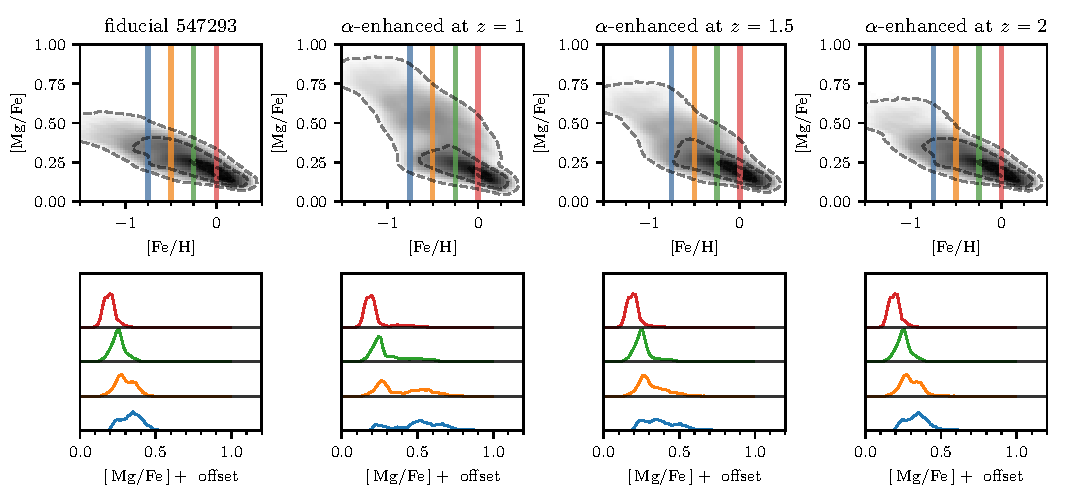
\includegraphics[width=\textwidth]{ch4/app_547293.pdf}
  \caption{The same as Figure~\ref{fig:app0}, but for a random galaxy from our initial catalog.}
  \label{fig:app15}
\end{figure*}

\begin{figure*}
  \centering
  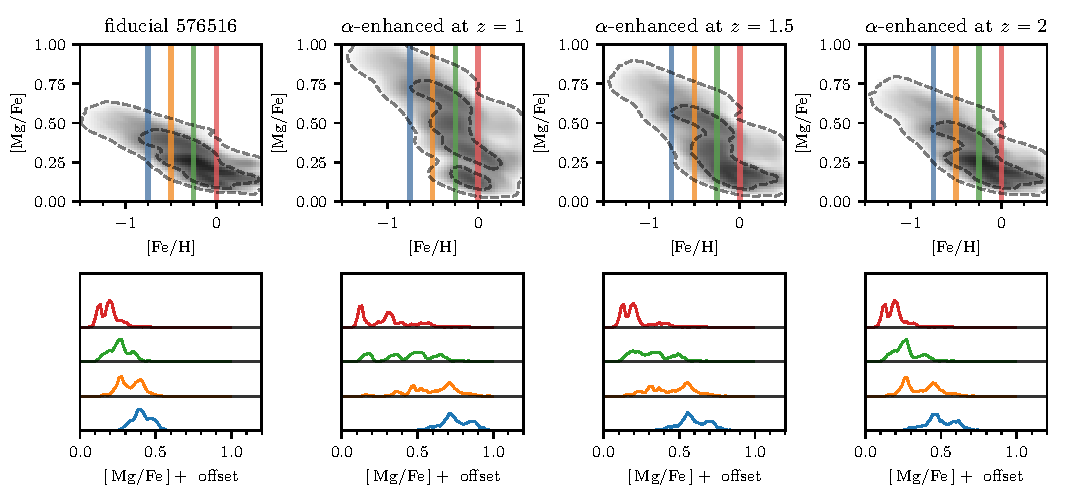
\includegraphics[width=\textwidth]{ch4/app_576516.pdf}
  \caption{The same as Figure~\ref{fig:app0}, but for a random galaxy from our initial catalog.}
  \label{fig:app16}
\end{figure*}

\chapter{The Emergence of Human Consciousness}
\begin{adjustwidth}{.8cm}{0cm}
\textit{Three things can not hide for long: the Moon, the Sun and the Truth.}

\hspace{9cm} -- Siddhartha Gautama
\end{adjustwidth}

\noindent
We now broaden our interests considerably. One of the great mysteries of our time is that the sun and moon have approximately the same apparent diameter on the sky, an apparent coincidence. However, because the moon is receding from the Earth, a more precise statement is that the coincidence is between the timing of the emergence of human consciousness at a time when the sun and moon have the same apparent diameter.

A natural outcome of the similar size of the sun and moon is the presence of total solar eclipses. However, because they have such similar sizes on the sky, total solar eclipses are quite rare, occurring about once every 375 years for a given spot on Earth \citep[varying somewhat with latitude][]{2002mmam.book.....M}. Given the current recession rate of the moon of $\sim3.8\,\textrm{cm}/\textrm{yr}$, the semi-major axis of the moon would have been $\sim0.02\,\%$ smaller when \textit{Homo erectus} emerged $\sim2\,\Myr$ ago, implying a very minor change to the overall occurrence of total solar eclipses. Assuming a generational turnover of $20\,\textrm{yr}$ \citep{homoerectus_lifespan}, this means that \textit{H. erectus} on average witnessed a solar eclipse about once every 18 generations.\footnote{This estimate is agnostic to whether they had a nomadic or sedentary lifestyle, since any movement patterns would be uncorrelated with impending eclipses. Note also that a given lineage from $2\,\Myr$ ago to the present would encounter about 5k eclipses, assuming 20~years between each generation.} This begs the question of how they would interpret such an event, and if it may lead to any appreciable effect on their long-term evolutionary outcome.

The answer is likely not, but it is even more likely that no one is still reading, so we can continue. Does witnessing totality confer any advantage for the emergence of consciousness? Because there is no genetic bias towards who would witness an eclipse, the effect must be of second-order. As an illustrative example, the attempt of a small child to understand an eclipse might push their brain to develop a slightly higher mental capacity. Some children will be able to develop this capacity at a higher rate than others because of random genetic mutations, and it is those children who are conferred an evolutionary advantage. The fact these events happen on generational timescales only enforce their power.

To be clear, this proposition is by no means a direct cause and effect argument. It is clearly not the case that consciousness emerged during the first-ever solar eclipse. However, the fact that the sun and moon have the same apparent size on the sky, and that solar eclipses happen regularly but with an occurrence that makes them a powerful and mysterious event, may have made the arising of consciousness go from being a $20\sigma$ event to an $18\sigma$ event.

\end{appendices}
